\documentclass[12,french]{report}
\usepackage{geometry}
\geometry{vmargin=3cm, hmargin=3cm}
\usepackage[T1]{fontenc}
\usepackage[utf8]{inputenc}
\usepackage[french]{babel}
\usepackage{graphicx}
\usepackage{amsmath}
\usepackage{amssymb}
\usepackage{sectsty}
\usepackage{authblk}
\usepackage{algpseudocode}
\usepackage{algorithm}
\usepackage{xspace}
\usepackage{mathtools}
\usepackage{mathrsfs}
\usepackage{enumitem}
\usepackage{titlesec}
\usepackage{hyperref}
\usepackage{xcolor}
\usepackage[justification=centering]{caption}
\usepackage{float}
\usepackage{tabto}

\usepackage{listings}
\usepackage{cleveref}

\renewcommand{\lstlistingname}{Code}
%\renewcommand{\figurename}{Fig.}

\lstdefinestyle{chstyle}{%
backgroundcolor=\color{gray!12},
basicstyle=\ttfamily\small,
showstringspaces=false,
numbers=left}

%\AddThinSpaceBeforeFootnotes
%\FrenchFootnotes

\titleformat{\chapter}[hang]{\bf\Huge}{\thechapter.}{2pc}{}
\titlespacing*{\chapter}{10pt}{0pt}{40pt}[0pt]
\newcommand{\HRule}{\rule{\linewidth}{0.5mm}}

\providecommand{\keywords}[1]{\textbf{\textit{Keywords:}} #1}
\bibliographystyle{apalike}

\usepackage{hyperref}

\begin{document}
\hypersetup{pdfborder=0 0 0}

\begin{titlepage}

\begin{center}
	\vspace*{\stretch{1}}	
	\textsc{{\LARGE Institut national des sciences appliquées de Rouen} \\ 			\vspace{6mm} {\Large INSA de Rouen}} \\
	\vspace{5mm}
	
\includegraphics[width=0.4\textwidth]{./Images_pooa/insa}\\[1.0 cm]

	\textsc{\Large Projet POOA GM4}\\[0.6cm]

	% Title
	\HRule \\[0.5cm]
	{ \Huge \bfseries Réalisation d'un Tricount en java}\\[0.2cm]
	\HRule \\[0.75cm]

	
\includegraphics[width=0.7\textwidth]{./Images_pooa/Tricount}\\[0.9 cm]

	% Author and supervisor
	\begin{minipage}{0.4\textwidth}
		\begin{flushleft} \large
			\emph{Auteurs:}\\
			Thibaut \textsc{André-Gallis} \\
			{\small\href{mailto:thibaut.andregallis@insa-rouen.fr}{thibaut.andregallis@insa-rouen.fr}} \\
			Kévin \textsc{Gatel} \\
			{\small\href{mailto:kevin.gatel@insa-rouen.fr}{kevin.gatel@insa-rouen.fr}}\\
			Hugo \textsc{Merelle} \\
			{\small\href{mailto:hugo.merelle@insa-rouen.fr}{hugo.merelle@insa-rouen.fr}}\\
			Marion \textsc{Mesnil} \\
			{\small\href{mailto:marion.mesnil@insa-rouen.fr}{marion.mesnil@insa-rouen.fr}}\\
		\end{flushleft}
	\end{minipage}
	\begin{minipage}{0.4\textwidth}
		\begin{flushright} \large
			\emph{Enseignants:} \\
			Cecilia \textsc{Zanni-Merk} \\
			{\small\href{mailto:cecilia.zanni-merk@insa-rouen.fr}								{cecilia.zanni-merk@insa-rouen.fr}}\\
		\end{flushright}
	\end{minipage}
	\vspace*{\stretch{1}}

	\vfill
	{\large 4 janvier 2022}
\end{center}
\end{titlepage}

\tableofcontents
\listoffigures

\renewcommand{\chaptername}{}
\chapter*{Introduction}

Tricount est une application qui permet d'organiser les dépenses de groupe. Ses utilisations sont multiples, elle permet notamment la répartition équitable des dépenses du groupe et le fait de pouvoir rembourser facilement quelqu'un si besoin. Elle peut également faire l’objet d’un récapitulatif de compte.\\

Dans ce projet on se propose de réaliser un Tricount à notre échelle, c'est -à -dire une application “locale” entre plusieurs clients (6 maximum) et un serveur. Le terme local est utilisé dans le sens où les clients peuvent se connecter au serveur s'ils partagent le même réseau.\\

L’utilisateur qui lance le serveur est appelé administrateur. Lui et lui seul a le droit d’ouvrir et/ou fermer l’application lorsqu’il le souhaite. Les autres utilisateurs ne peuvent se connecter à l’application que lorsque le serveur est ouvert au préalable par l’administrateur. \\

Lorsque le serveur est fermé toutes les données sont perdues. Nous ne stockons pas les données en local, tout se fait dans le serveur lorsqu’il est ouvert.\\

Dans un premier temps, nous allons voir différents diagrammes afin de clarifier la manière d’aborder le sujet. Puis dans un second temps, nous allons implémenter l’application en Java et commenter les éventuelles difficultées rencontrées.\\


\chapter{UML Spécification}

\section{Cas d'utilisation}

\begin{figure}[H]
	\center
	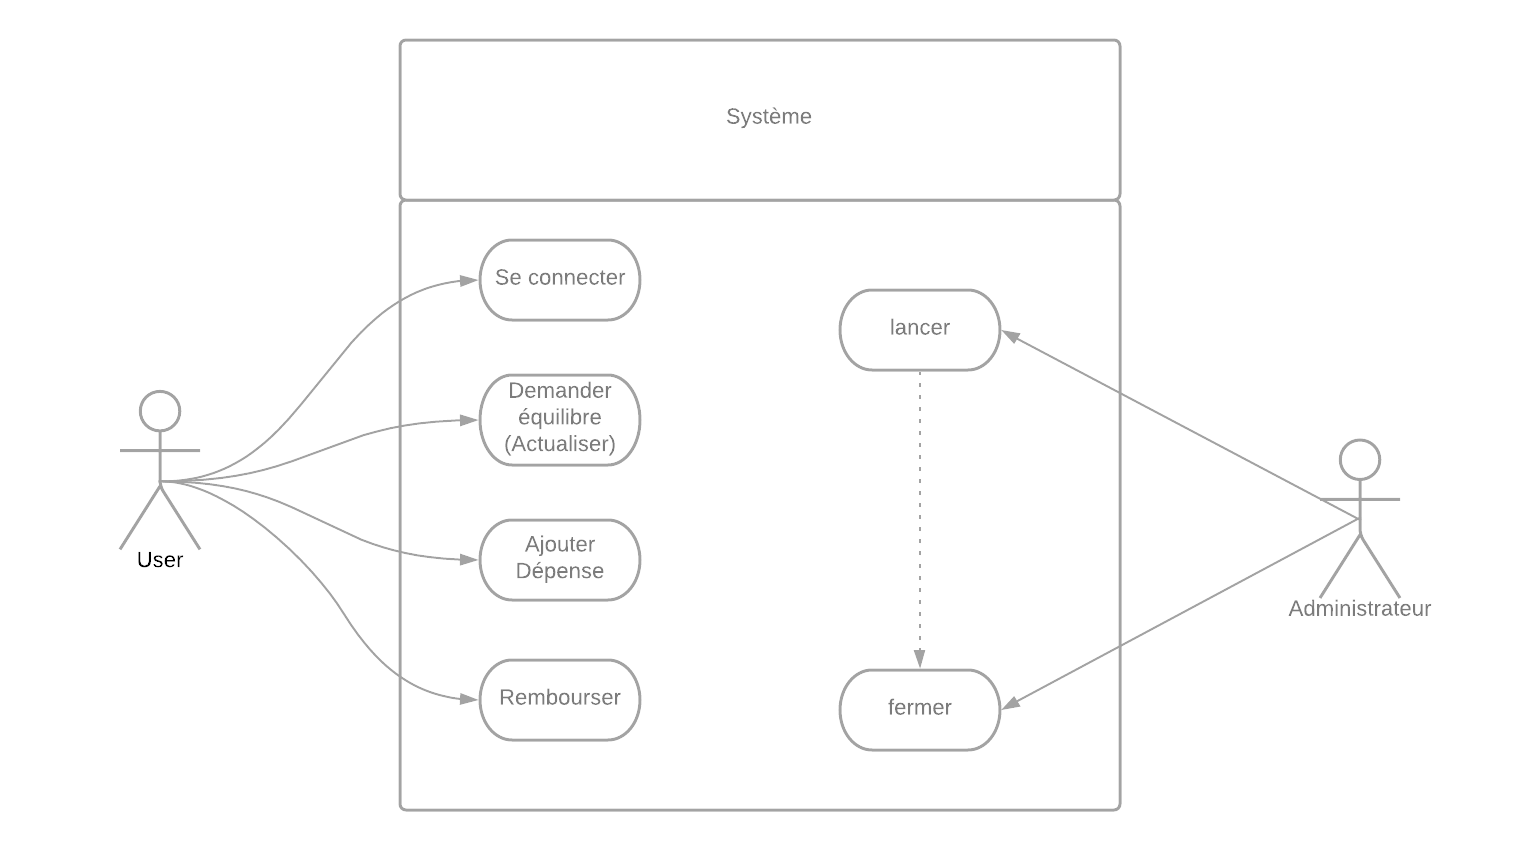
\includegraphics[width=0.7\textwidth]{./Images_pooa/Use-Case}
	\caption{Diagramme de cas d'utilisation}
\end{figure}\vspace{0.2cm}

Dans ce diagramme on distingue les deux cas suivants : l’administrateur et l’utilisateur de l’application. Le premier permet de lancer l’application puis de l'arrêter, alors que les “users” utilisent l’application suivant quatre options lorsque cette dernière est bien lancée.


\section{Séquence}

Le diagramme de séquence représentant l’option “Se connecter” pour l’utilisateur est représenté sur chacun des trois diagrammes de séquence suivants.\\

Le diagramme de séquence de l’option “Demander équilibre (Actualiser)” est le suivant :\\


\begin{figure}[H]
	\center
	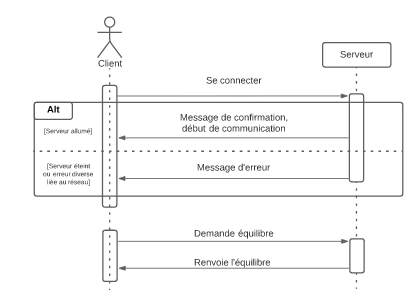
\includegraphics[width=0.7\textwidth]{./Images_pooa/Sequence_1}
	\caption{Diagramme de séquence "Demander Equilibre (Actualiser)"}
\end{figure}\vspace{0.2cm}

Afin de pouvoir “Demander équilibre” au serveur, nous devons nous assurer que l’utilisateur est connecté au serveur. Dans le cas où l’utilisateur est bien connecté, un message de confirmation est envoyé à l’utilisateur et la requête peut commencer à être traitée, dans le cas contraire un message d’erreur est envoyé et la requête est renvoyée. Si l’utilisateur est correctement connecté au Serveur alors le Serveur envoie la liste des utilisateurs de l’application à l’utilisateur en les informant s’ils sont “en avance” ou “en retard” par rapport aux autres utilisateurs selon une somme d’argent indiquée.\\


Le diagramme de séquence de l’option “Ajouter dépense” est le suivant :\\

\begin{figure}[H]
	\center
	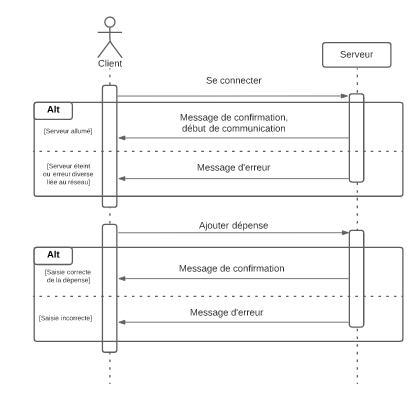
\includegraphics[width=0.7\textwidth]{./Images_pooa/Sequence_2}
	\caption{Diagramme de séquence "Ajouter dépense"}
\end{figure}\vspace{0.2cm}

Même chose que pour “Demander équilibre” l’utilisateur doit être connecté à l’application afin de pouvoir demander cette requête au Serveur. La dépense doit être positive et l’utilisateur doit au moins “cocher” une personne sur les 6 de manière à répartir la dépense équitablement. Le cas où l’utilisateur “coche” uniquement lui-même doit être rejeté. Un message de confirmation est envoyé à l’utilisateur si la requête s’est bien passée, un message d’erreur est retourné dans le cas contraire.\\

Le diagramme de séquence de l’option “Rembourser” est le suivant :\\

\begin{figure}[H]
	\center
	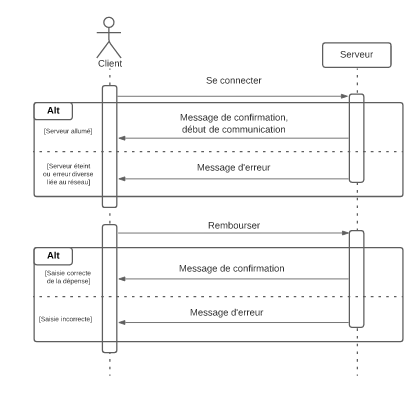
\includegraphics[width=0.7\textwidth]{./Images_pooa/Sequence_3}
	\caption{Diagramme de séquence "Rembourser"}
\end{figure}\vspace{0.2cm}

De la même manière que les précédents, l’utilisateur doit être connecté à l’application afin de pouvoir demander cette requête au Serveur. La somme du remboursement doit être également positive, et l’utilisateur doit “cocher” une et une seule personne (pas lui même) afin de le rembourser. Un message de confirmation est envoyé à l’utilisateur si la requête s’est bien déroulée, un message d’erreur est retourné dans le cas contraire.

\section{Modèle du domaine}

Nous avons réalisé le diagramme de modèle du domaine suivant :\\

\begin{figure}[H]
	\center
	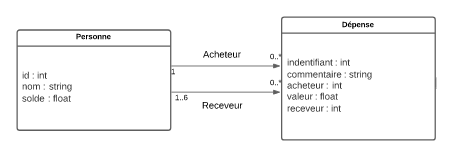
\includegraphics[width=0.7\textwidth]{./Images_pooa/Modele}
	\caption{Diagramme de modèle du domaine}
\end{figure}\vspace{0.2cm}

Comme on peut le voir ci-dessus on peut distinguer 2 classes \textit{Personne} et \textit{Dépense} qui sont liées entre elles. Commençons d’abord par nous intéresser à chacune d’entre elles :\\

\begin{itemize}[label=\textbullet]
	\item \emph{Personne} :
La classe Personne représente un utilisateur de l’application tricount. Il va donc posséder deux variables d’instances, son nom qui sera une chaîne de caractères et son solde représenté par un flottant.
	\item \emph{Dépense} :
La classe dépense représente une dépense évidemment mais plus particulièrement une transaction entre deux personnes. Elle est définie par 5 variables : son identifiant qui sera un entier, un commentaire qui décrira à quoi correspond dans la vraie vie cette dépense (ex tickets de bus), une valeur flottante et puis un acheteur et un receveur qui seront des personnes.
\end{itemize}\vspace{0.5cm}


Ces deux classes sont liées car une dépense relie deux personnes l’une acheteuse et l’autre receveuse. S’il n’y a pas d’acheteur alors il ne peut y avoir de dépense. Chaque dépense est liée à uniquement un acheteur et un receveur. Cependant un acheteur peut avoir effectué plusieurs dépenses et un receveur en avoir reçu plusieurs également. 
Il est nécessaire de préciser que dans notre cas nous avons décidé de considérer le receveur comme une seule personne mais nous allons également traiter le cas où une dépense concerne plusieurs receveurs en générant plusieurs dépenses qui posséderont le même identifiant et qui auront une valeur divisée par le nombre de receveurs. Chacune reliera l’acheteur et un des receveurs. 

\section{Maquette de l'application}

\begin{figure}[H]
	\center
	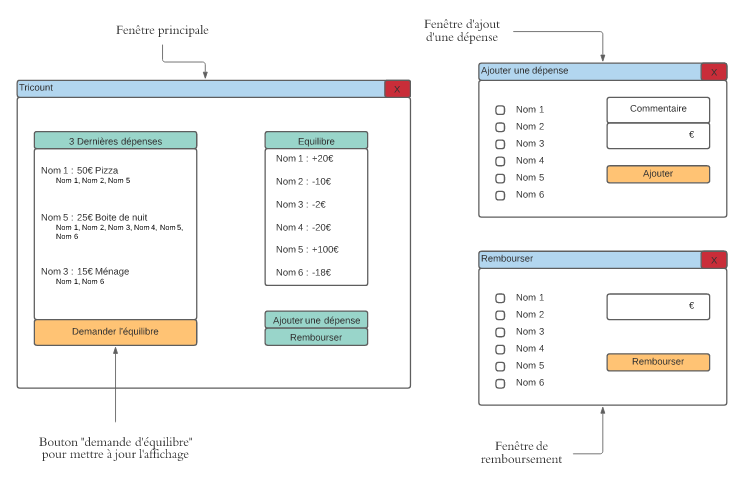
\includegraphics[width=0.7\textwidth]{./Images_pooa/Maquette}
	\caption{Maquette de l'application}
\end{figure}\vspace{0.2cm}

Elle peut être expliquée par le diagramme de navigation suivant.

\section{Navigation}

\begin{figure}[H]
	\center
	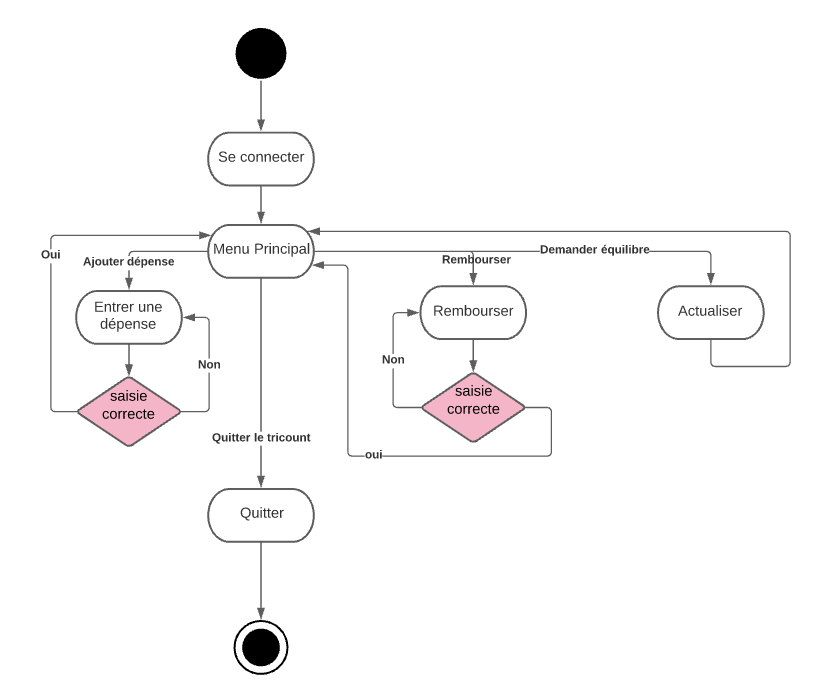
\includegraphics[width=0.7\textwidth]{./Images_pooa/Navigation}
	\caption{Diagramme de navigation}
\end{figure}\vspace{0.2cm}

L’utilisateur ouvre le tricount et se connecte, il arrive alors sur la fenêtre principale : le “menu principal”. Il peut donc entrer une dépense en cliquant sur le bouton “Ajouter une dépense”. Il arrive ensuite sur la fenêtre d’ajout d’une dépense et peut entrer le montant de sa dépense et sélectionner les personnes qui participent à cet achat (il peut se sélectionner lui-même si il paie également). Il clique ensuite sur “Ajouter”. Si sa saisie est correcte la dépense est prise en compte et il retourne sur la fenêtre principale, sinon un message d’erreur apparaît et il doit refaire sa saisie.
Le principe est le même pour le remboursement.
Ensuite, si l’utilisateur sélectionne le bouton “Actualiser” l’affichage s’actualise avec les dernières dépenses (et les derniers participants s'ayant connectés entre temps).
Enfin, pour quitter le tricount il suffit de cliquer sur la croix rouge en haut à gauche de la fenêtre principale.\\

La fonction principale est :\\

\begin{itemize}[label=\textbullet]
	\item \textit{public void AddDepense(Int id, String Com, Personne acheteur, Int Val, Personne receveur) throws RemoteException;}
Elle permet d’ajouter une dépense et de rembourser ( en faisant une dépense inverse). Les dépenses sont stockées dans un tableau comme vu dans les premiers TDs. Une dépense à un client et un acheteur. Lorsque une dépense est crée elle sera automatiquement stockée plusieurs fois (le nombre de participant à la dépense).
\end{itemize}\vspace{0.5cm}

Pour notre Programme nous aurons deux utilisateurs :\\

\begin{itemize}[label=\textbullet]
\item L’administrateur qui lance et ferme le serveur.\\
\item Et les utilisateurs qui se connectent dans un premier temps. Puis ils ont 3 possibilitées:\\
	\begin{itemize}
	\item Actualiser les soldes (l’équilibre de chaque personne)\\
	\item Rembourser un autre utilisateur.\\
	\item Ajouter une dépense.\\
	\end{itemize}
\end{itemize}


\chapter{UML Conception}

\section{Interaction}

On retrouve dans un premier temps le diagramme d'interaction pour la requête "Ajouter dépense" :

\begin{figure}[H]
	\center
	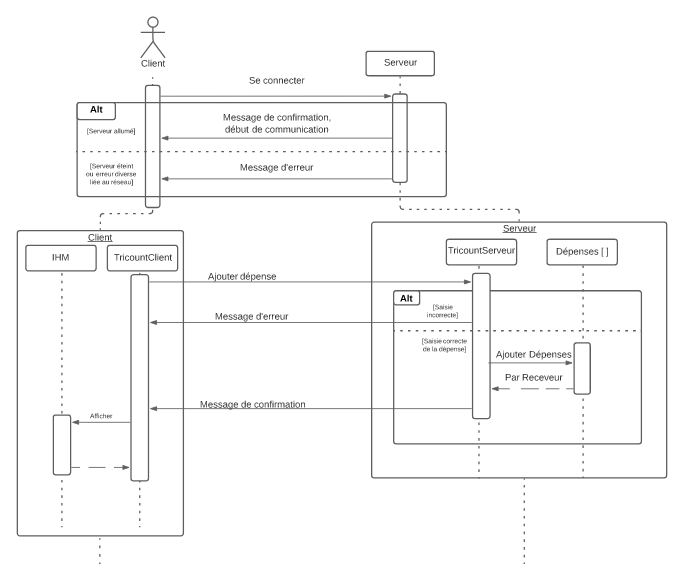
\includegraphics[width=0.7\textwidth]{./Images_pooa/Interaction_AjouterDepense}
	\caption{Diagramme d'interaction "Ajouter dépense"}
\end{figure}\vspace{0.2cm}

On a exactement le même principe que pour le diagramme de séquence. On vérifie d’abord la connexion puis le TricountClient (main) fait une requête d’ajout de dépense au TricountServeur. Dans un premier temps, le Serveur vérifie la saisie. Si cette dernière est incorrecte un message d'erreur est envoyé au client. Si la saisie est correcte alors le serveur ajoute les dépenses au tableau stockées dans TricountServeur. Plus d'informations sont données dans la section Clarification plus bas.
Une fois le message de confirmation envoyé, l'IHM est actualisée (la fenêtre est fermée). \\

\begin{figure}[H]
	\center
	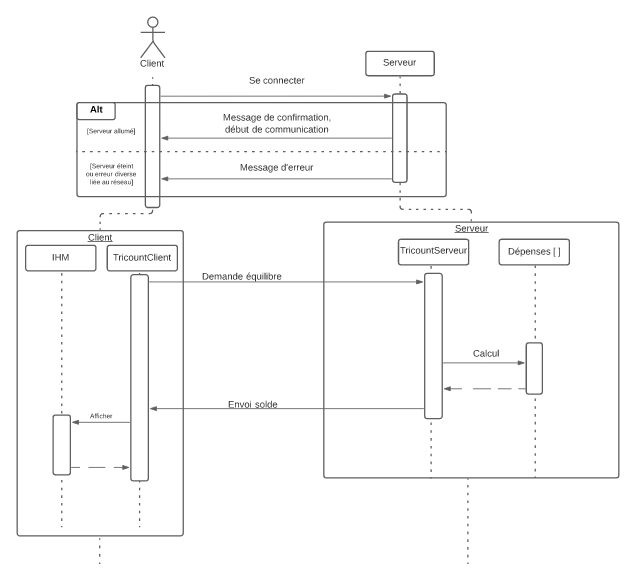
\includegraphics[width=0.7\textwidth]{./Images_pooa/Interaction_DemanderEquilibre}
	\caption{Diagramme d'interaction "Demander Equilibre (Actualiser)"}
\end{figure}\vspace{0.2cm}

Pour le calcul d'équilibre le principe est similaire au cas précédent. La connexion est vérifiée dans un premier temps et une requête est envoyée par le Client. Ici aucune vérification de saisie n'est nécessaire car l'utilisateur n'a rien à entrer (il clique sur un bouton). Le calcul est effectué côté serveur, encore une fois le détail de calcul est rédigé dans la section Clarification. Une fois le calcul effectué, le résultat est envoyé au TricountClient. Ce dernier met à jour son IHM afin de montrer à l'utilisateur les nouveaux chiffres. \\

\begin{figure}[H]
	\center
	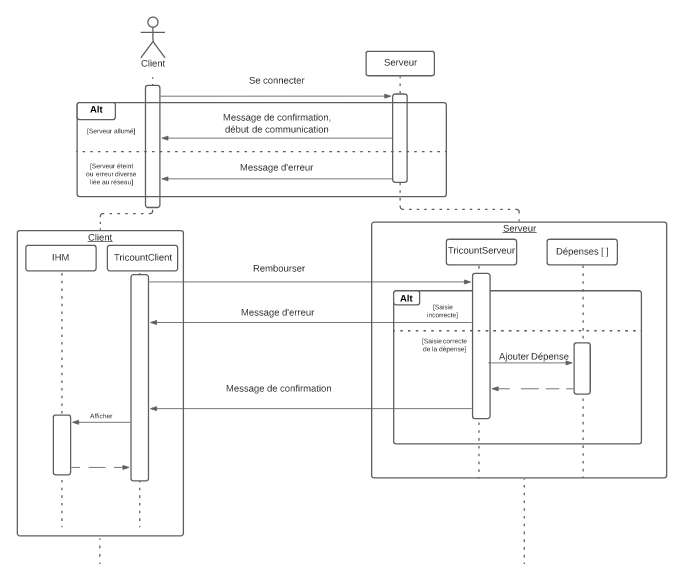
\includegraphics[width=0.7\textwidth]{./Images_pooa/Interaction_Rembourser}
	\caption{Diagramme d'interaction "Rembourser"}
\end{figure}\vspace{0.2cm}

Pour le remboursement on effectue la même chose que pour l'ajout de dépenses. Encore une fois vous trouverez plus d'informations dans la section Clarification. 

\section{Classes}

Afin de séparer le Serveur et le Client nous avons décidé de faire un diagramme de classe pour chacun des deux.

\begin{figure}[H]
	\center
	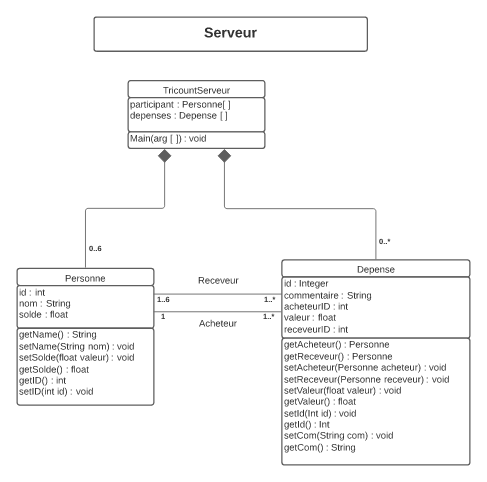
\includegraphics[width=0.7\textwidth]{./Images_pooa/Diagramme_de_classe_Serveur}
	\caption{Diagramme de classe coté Serveur}
\end{figure}\vspace{0.2cm}

Du coté serveur il y aura donc 3 classes pour implémenter ce Tricount. \\

\begin{itemize}[label=\textbullet]
\item La première est \textit{TricountServeur} qui contient le main. Ce sera l’administrateur qui ouvrira et fermera l’application (le serveur) pour permettre ainsi aux clients de s’y connecter par la suite. Elle contient comme attributs un tableau de \textit{Personne} (de taille 6) qui contient tous les participants, et un tableau dynamique de \textit{Depense} regroupant ainsi toutes les dépenses ajoutées depuis le début.\\

\item La classe \textit{Personne} contient le nom et le solde du participant. L’id différente pour chaque personne va permettre de reconnaître deux personnes dans la situation où ils possèdent le même solde et le même nom.\\

\item Enfin la classe \textit{Depense} va avoir comme attribut l’id de la personne qui achète et l’id de la personne qui reçoit la dépense. Pour la même raison, on stockera également une id différente pour chaque dépense pour les reconnaître. On rappelle que s’il y a plusieurs receveurs, il suffit simplement de créer autant de dépenses qu’il y a de receveur pour le même acheteur (Voir la partie clarification un peu plus bas). Enfin on a évidemment le commentaire de la dépense et la valeur de cette dernière.\\
\end{itemize}

On remarque bien sur le diagramme que les classes \textit{Depense} et \textit{Personne} dépendent du \textit{ServeurTricont}. Une dépense a bien un seul acheteur avec plusieurs receveurs et chaque personne a son tableau dynamique de dépense.\\

\begin{figure}[H]
	\center
	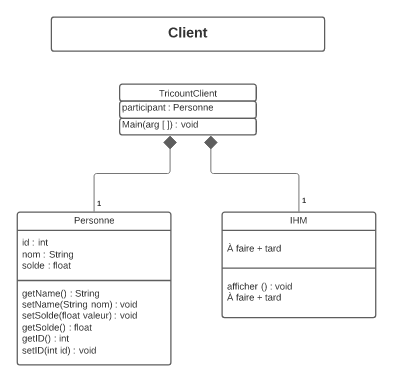
\includegraphics[width=0.7\textwidth]{./Images_pooa/Diagramme_de_classe_Client}
	\caption{Diagramme de classe coté Client}
\end{figure}\vspace{0.2cm}

Du côté Client c’est assez similaire. On retrouve deux classes \textit{Personne} et \textit{IHM} qui dépendent de la classe main \textit{TricountClient}. Cette classe \textit{TricountClient} va en réalité chercher à se connecter un Serveur. Le serveur ici est la classe vue précédemment \textit{ServeurTricount}. Une fois le Client connecté, la personne associée aura sa propre interface graphique et va pouvoir ainsi visualiser les dépenses de chacun, calculer l’équilibre ou encore ajouter une dépense. Ceci prend fin lorsque le serveur est fermé.\\

Ayant implémenté une interface homme-machine (IHM) nous avons également réalisé un diagramme de classe de ce dernier :

\begin{figure}[H]
	\center
	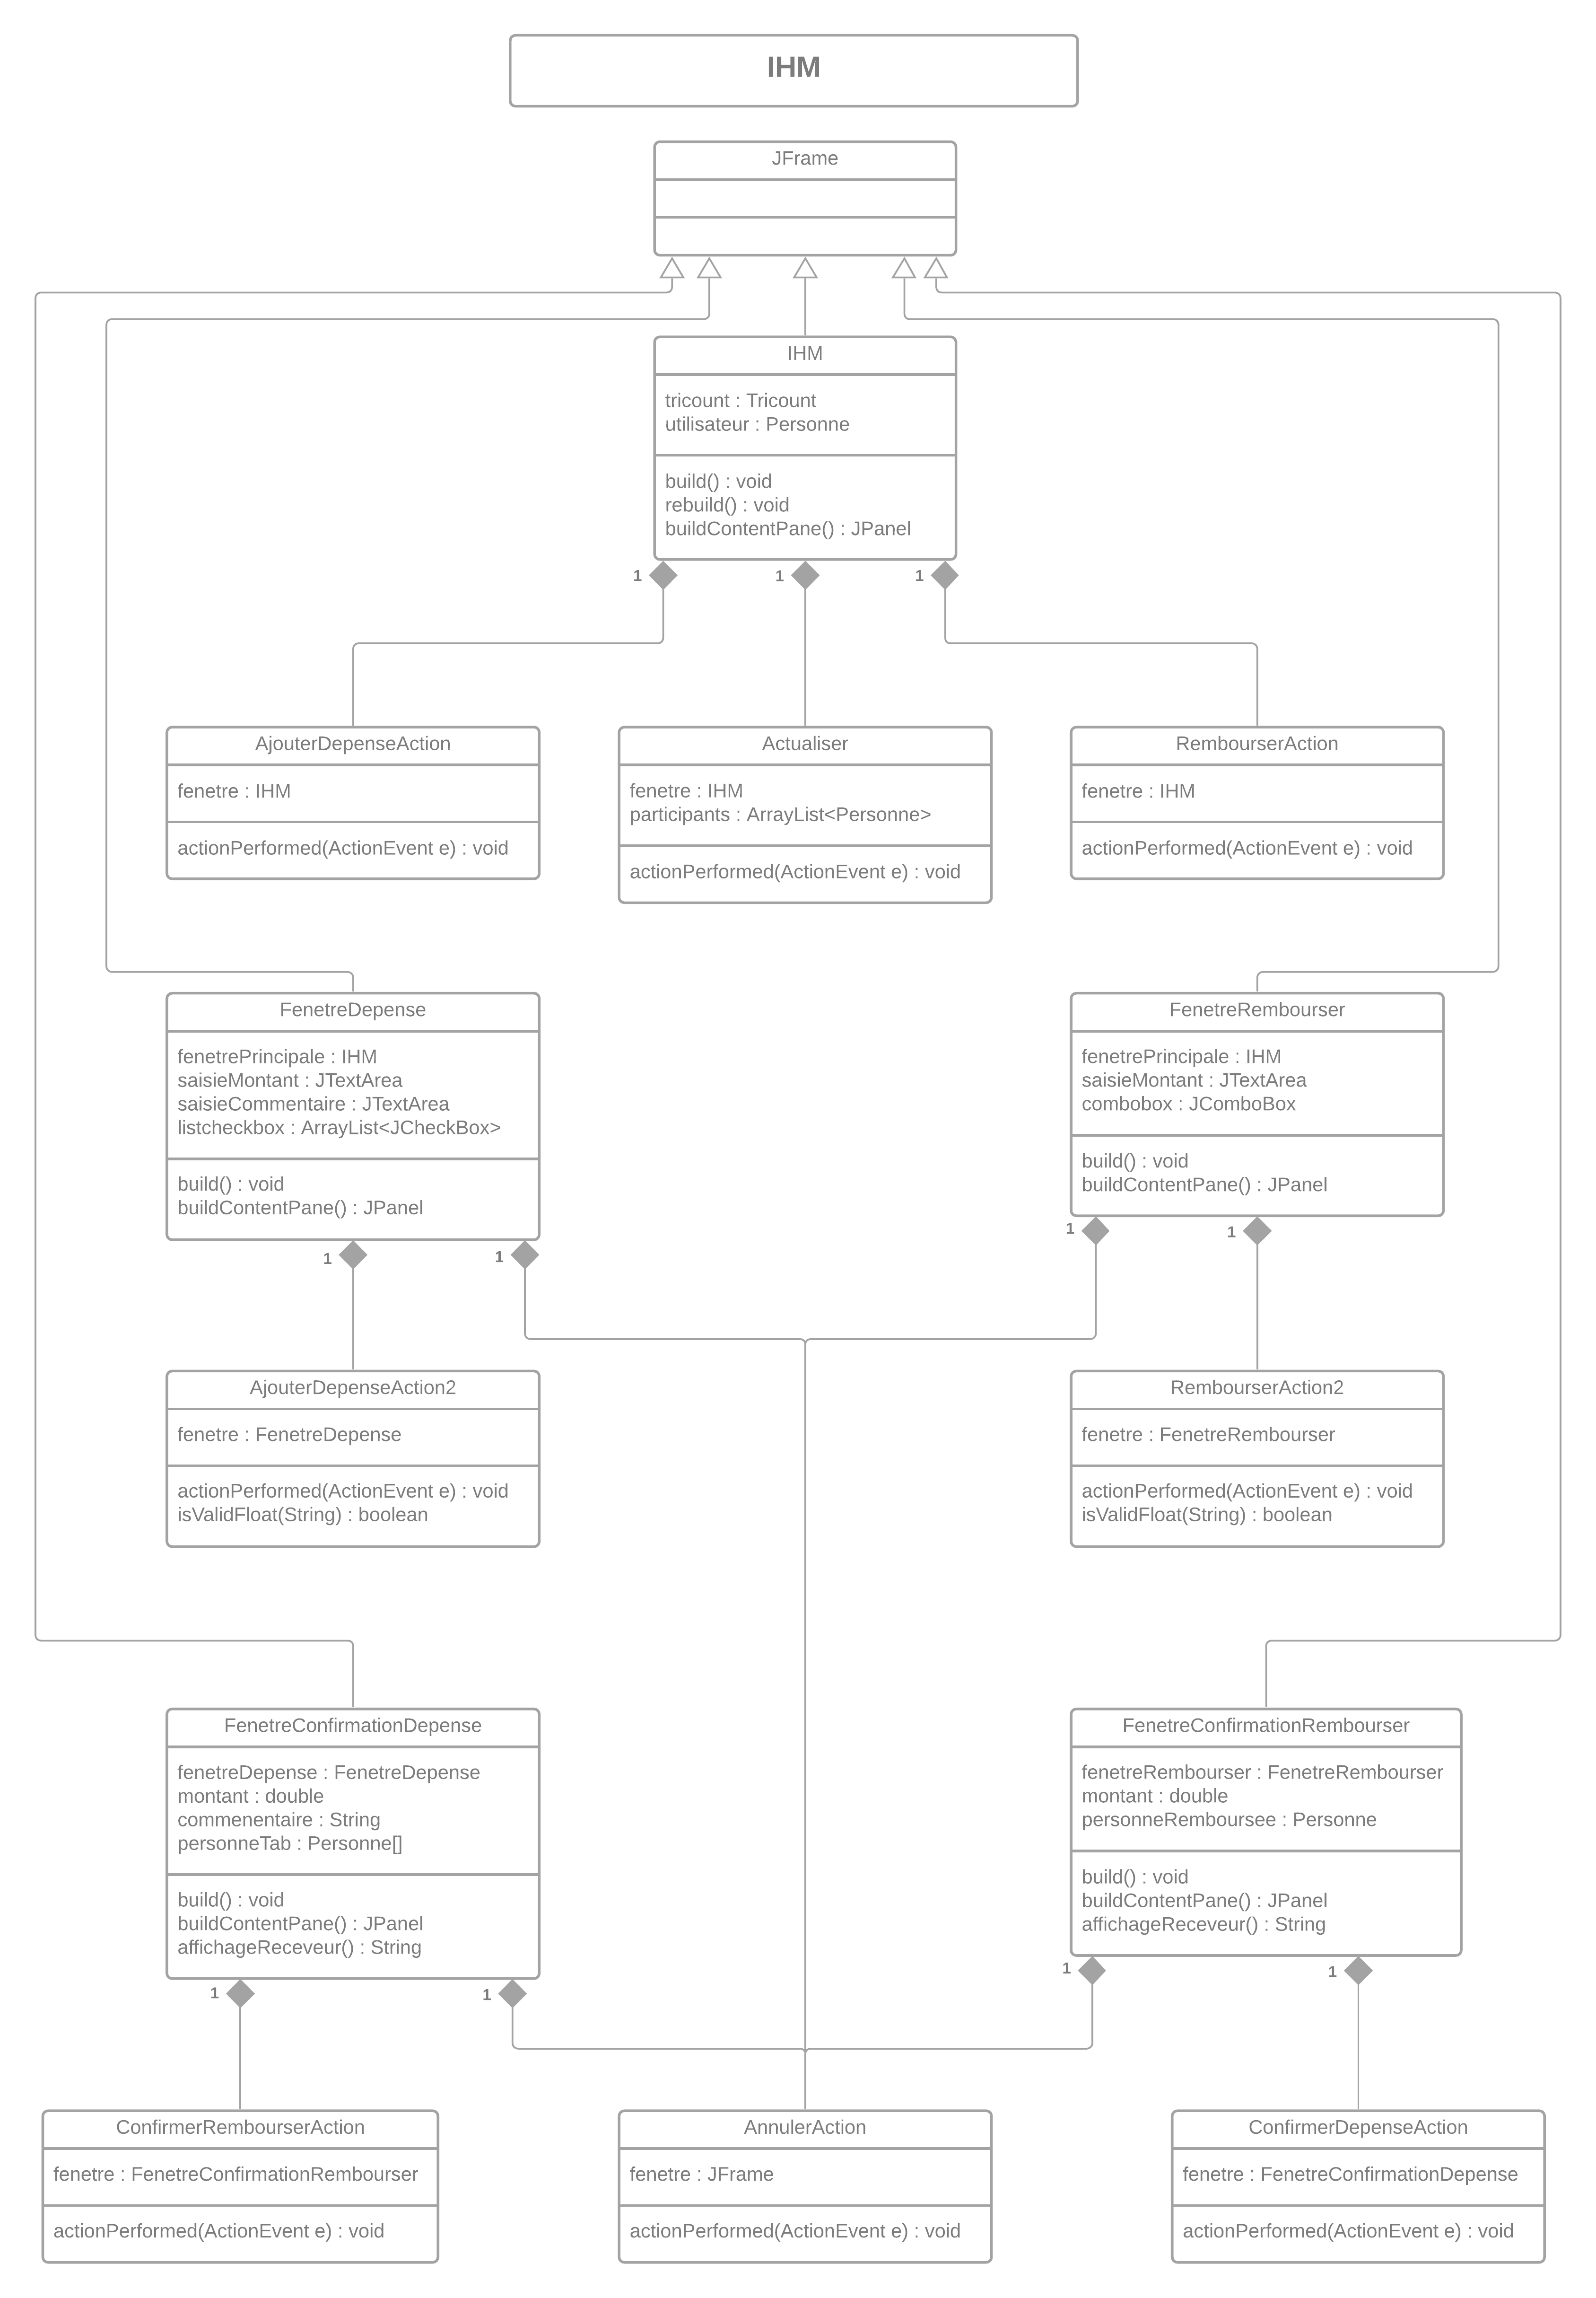
\includegraphics[width=0.9\textwidth]{./Images_pooa/Diagramme_de_classe_IHM}
	\caption{Diagramme de classe IHM}
\end{figure}\vspace{0.2cm}

Il s'agit essentiellement de manipulations de JFrame et de JPanel sous toute leurs formes, en ajoutant à cela des boutons permettant d'ouvrir ou de fermer les fenêtres. L'interface est légèrement différente de la maquette.

\section{Paquetage}

Nous avons regroupé les éléments de cette façon : \\

\begin{figure}[H]
	\center
	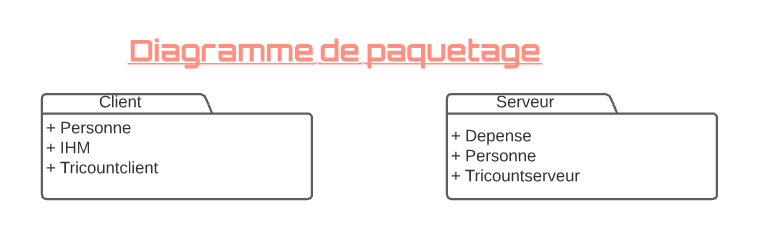
\includegraphics[width=0.7\textwidth]{./Images_pooa/Paquetage}
	\caption{Diagramme de paquetage}
\end{figure}\vspace{0.2cm}

Le client contient \textit{TricountClient} qui est sa classe principale (le “main”), un IHM sur lequel il pourra naviguer dans l’application et la classe Personne qui décrit le client en question. 
Le serveur contient la classe Dépense puisqu’il gère l’affichage des dépenses et le calcul de l’équilibre. La classe TricountServeur est sa classe principale (le “main”) et la classe Personne lui permet d’associer une dépense à des personnes et de modifier leur solde.

\section{Composants}

Le découpage de composants est représenté comme suit :\\

\begin{figure}[H]
	\center
	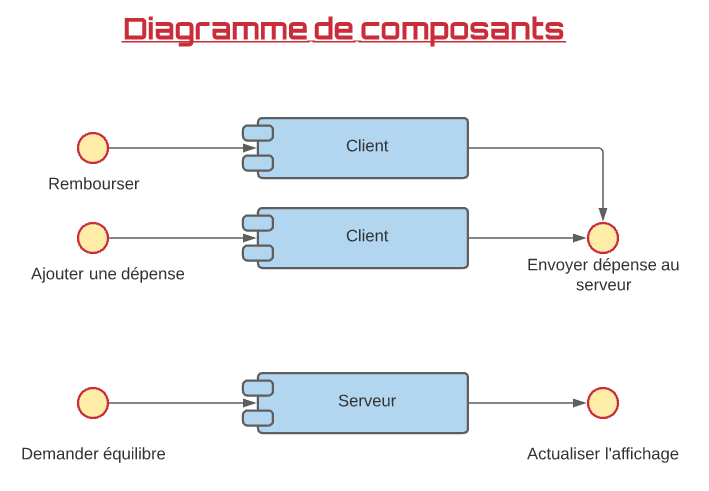
\includegraphics[width=0.7\textwidth]{./Images_pooa/Composants}
	\caption{Diagramme de composants}
\end{figure}\vspace{0.2cm}

Un client peut ajouter une dépense et rembourser quelqu’un. Cette demande est ensuite envoyée au serveur avec le montant et les autres caractéristiques d’une dépense. 
La demande d’équilibre peut également être demandée au serveur qui, par la suite, va actualiser l’affichage. 

\section{Déploiement}

\begin{figure}[H]
	\center
	\includegraphics[width=0.7\textwidth]{./Images_pooa/Déploiement}
	\caption{Diagramme de composants}
\end{figure}\vspace{0.2cm}

Nous avons également fait un diagramme de déploiement pour notre programme à la suite du diagramme de paquetage. \\

Notre diagramme se décompose en 2 entités : 
\begin{itemize}[label=\textbullet]
\item \textbf{Le client} ou utilisateur qui possède son ordinateur et qui de son côté ne verra que l’IHM après s’être connecté au serveur du Tricount. Il pourra depuis son poste ajouter une dépense ou un remboursement ainsi que demander l’équilibre du Tricount.\\
\item \textbf{L’administrateur} qui va s’occuper du serveur qui sera sur un autre appareil que le client. L’administrateur après avoir lancé le serveur permettra au client de s’y connecter et d’effectuer les actions listées précédemment. 

\end{itemize}\vspace{0.2cm}

Nous aurons donc au moins deux ordinateurs distincts pour ce projet.

\chapter{Clarification pour l'implémentation}

\begin{itemize}[label=\textbullet]
\item \textbf{Stockage des dépenses} : Lors de la création d’une dépense on vient ajouter plusieurs objets au tableau dépenses. Par exemple:
Si Paul achète pour 45€ de pizza avec Eugène et Charles.
Dans ce cas, on crée 3 dépenses avec le même ID pour pouvoir savoir qu’ils sont liées. Ces trois dépenses ont un montant de 45/3=15€ ils ont l’ID de Paul comme acheteur et l’ID de Eugène, Charles et Paul.\\

\item \textbf{Equilibre}:
Pour calculer l’équilibre il suffit de sommer les montants où l’identifiant apparaît en tant qu’acheteur. Et ensuite soustraire les moments où l’identifiant est en receveur.
Exemple: Dans le cas où Paul achète pour 45€ de pizza avec Eugène et Charles. Si on calcule le cas de Paul on a donc -15 pour sa dépense et ensuite +15*3 dans les 3 dépenses où il est acheteur. Paul aura donc +30 par rapport aux autres.

\item \textbf{Remboursement}:
Pour effectuer un remboursement on doit juste ajouter une dépense “en inverse”. Si Paul a remboursé 10€ à Michel dans ce cas on crée une dépense de Paul (acheteur) à Michel (receveur) d’un montant de 10€.

\end{itemize}

\chapter{Problèmes rencontrés durant l'implémentation}

Même si à premiers regards nous pensions que ce projet serait assez simple et rapide vu la simplicité de l'application que tout le monde connaît, il s'en est suivi quelques surprises lors de l'implémentation. En effet ce fut la première fois que nous manipulions le RMI sous forme de projet, et que de plus l'IHM devait gérer les échanges Serveur-Client et Client-Serveur.\\

La première difficulté fut le temps. En effet ne pouvant pas commencer à programmer avant la validation de l'ensemble des diagrammes, il a fallu s'organiser de manière à être à jour sur les travaux du groupe et finir le projet en deux semaines.\\

La deuxième difficulté est très vite apparu lors de l'implémentation de l'IHM. Pour beaucoup d'entre nous, la manipulation des JFrame, JPanel, JButton en java ne nous étaient pas familier et il a fallu lire de nombreuses documentations afin de comprendre comment tout cela marchait. \\

Une fois l'IHM fini, le dernier problème fut de fusionner l'IHM avec le RMI. Lors de partage de code entre chacun d'entre nous grâce à l'outil Git, des fichiers ".class" ne se supprimaient pas ou n'était pas à jour avec un autre camarade ce qui entraînait des erreurs.\\

Toutes ces erreurs furent minimes et nous ont évidemment appris sur la manière de coder java en général et sur le RMI vu en cours.


\chapter*{Conclusion}

Pour commencer ce projet a été très formateur pour nous tous dans plusieurs domaines de la programmation.\\

Premièrement nous avons pu appliquer les nombreuses notions vues en cours sur notamment toute la partie conception avec laquelle nous n'étions pas si familier avant cela. Cela nous a permis de comprendre l'importance de la conception pré-implémentation surtout lorsque le projet se réalise en groupe. Nous avons pu nous familiariser d'avantages avec les nombreux diagrammes du modèle UML.\\
Nous avons également pu travailler sur un système de client serveur à distance et utilisant notamment le RMI, ce qui ne fût pas si simple à appréhender. En effet nous avons eu de nombreuses difficultés au cours du projet pour bien comprendre et utiliser toutes les nouvelles notions que cela impliquait, Cependant nous y sommes finalement parvenus grâce à l'échange entre les membres du groupes et les recherches et essais de chacun.\\
De plus Nous avons fais le chois d'ajouter une interface graphique à notre programme pour lui donner un aspect plus visuel et sympathique pour l'utilisateur et donc le rendre plus simple d'utilisation. Cela nous a demandé du travail supplémentaire pour développer l'IHM mais également pour la relier avec le RMI, mais nous sommes satisfait de l'aspect esthétique qu'il apporte au programme.\\

D'autre part nous étions tous familier avec l'application Tricount et nous avions tous une idée de comment elle fonctionnait. Mais nous ne savions pas comment l'implémenter sur un système client-serveur au lieu de tout sur une même machine. Il a fallu donc dans un premier temps nous mettre d'accord sur ce que nous allions faire à partir des idées de chacun. Puis ensuite de le développer parties par parties.\\

Pour conclure nous avons apprécié travailler sur ce projet qui comportait un sujet qui nous était familier mais avec des notions encore trop floues au départ, ce qui nous a permis de mieux comprendre et de savoir utiliser de nouveaux outils. La taille du groupe était plus importante qu'à notre habitude mais cela n'a pas posé de problèmes nous avions plus d'idées, cela demandait juste une phase plus clair de conception et de spécifications pour être sûr que nous allions tous dans la même direction au moment de commencer à implémenter nos parties respectives.\\
Si nous avions eu plus de temps nous aurions pu réfléchir à d'autres fonctionnalités à rajouter telle qu'une sauvegarde du tricount dans un fichier disponible sur le serveur pour pouvoir garder les tricount même lorsque tout le monde se déconnecte. 
Nous aurions pu aussi essayer de gérer plusieurs tricount en simultané pour permettre aux clients de rejoindre plusieurs tricount.


\end{document}
